\documentclass[12pt,a4paper,twocolumn]{article}

% ============================================================
% PACKAGES
% ============================================================
\usepackage[utf8]{inputenc}
\usepackage[T1]{fontenc}
\usepackage{lmodern}
\usepackage[margin=0.75in]{geometry}
\usepackage{graphicx}
\usepackage{xcolor}
\usepackage{hyperref}
\usepackage{listings}
\usepackage{amsmath,amssymb}
\usepackage{booktabs}
\usepackage{float}
\usepackage{tikz}
\usetikzlibrary{shapes.geometric, arrows.meta, positioning, fit, calc}
\usepackage{caption}
\usepackage{subcaption}
\usepackage{array}
\usepackage{multicol}
\usepackage{abstract}
\usepackage{fancyhdr}
\usepackage{enumitem}

% ============================================================
% CONFIGURATION
% ============================================================
\hypersetup{
    colorlinks=true,
    linkcolor=blue!70!black,
    urlcolor=blue!60!black,
    citecolor=green!50!black,
    pdftitle={Automated Hippocampal Volume Quantification Using U-Net},
    pdfauthor={Student}
}

\lstset{
    basicstyle=\ttfamily\scriptsize,
    breaklines=true,
    frame=single,
    backgroundcolor=\color{gray!8},
    keywordstyle=\color{blue!70!black}\bfseries,
    commentstyle=\color{green!50!black},
    stringstyle=\color{red!60!black},
    numbers=left,
    numberstyle=\tiny\color{gray},
    numbersep=3pt,
    tabsize=4
}

\pagestyle{fancy}
\fancyhf{}
\fancyhead[L]{\small Hippocampal Volume Quantification}
\fancyhead[R]{\small\thepage}

% ============================================================
% DOCUMENT BEGIN
% ============================================================
\begin{document}

% ============================================================
% TITLE
% ============================================================
\twocolumn[
\begin{@twocolumnfalse}
\begin{center}
{\LARGE\bfseries Automated Hippocampal Volume Quantification\\
from Brain MRI Using Deep Learning\\[0.4cm]}
{\large End-to-End Clinical AI Pipeline for Alzheimer's Disease Tracking\\[0.5cm]}

\textit{Udacity AI for Healthcare Nanodegree --- Course 3: 3D Medical Imaging}\\[0.3cm]
\textbf{Date: March 8, 2026}\\[0.3cm]
\rule{\textwidth}{0.5pt}
\end{center}

\begin{abstract}
This paper presents an end-to-end deep learning pipeline for automated hippocampal volume quantification from brain MRI scans. The hippocampus, a brain structure critical for memory formation, undergoes progressive atrophy in Alzheimer's disease, making volumetric measurement essential for diagnosis and monitoring. Our system employs a Recursive U-Net architecture trained on 260 annotated hippocampal volumes, achieving a mean Dice Similarity Coefficient of \textbf{0.900} and Jaccard Index of \textbf{0.820} on a held-out test set of 52 volumes. The pipeline includes data curation (NIFTI format), model training with multi-class segmentation (anterior/posterior hippocampus), and clinical deployment via DICOM/PACS integration. The deployed system processes incoming MRI studies automatically, generates standardized DICOM reports with volumetric measurements and clinical assessments, and integrates seamlessly into existing hospital Picture Archiving and Communication Systems (PACS). Inference runs in under 5 seconds on CPU, making it suitable for real-time clinical workflows.
\end{abstract}
\vspace{0.5cm}
\end{@twocolumnfalse}
]

% ============================================================
% 1. INTRODUCTION
% ============================================================
\section{Introduction}

Alzheimer's disease (AD) is the most common cause of dementia, affecting approximately 50 million people worldwide~\cite{who2019}. Hippocampal atrophy is one of the earliest and most reliable biomarkers for AD progression, with volume loss rates of 10--25\% per year in affected individuals~\cite{jack2010}.

Manual segmentation of the hippocampus from MRI scans by expert neuroradiologists requires 30--60 minutes per case and suffers from significant inter-rater variability. Automated segmentation using deep learning offers a scalable, consistent, and rapid alternative.

This work presents HippoVolume.AI, a complete clinical AI system consisting of three integrated components:
\begin{enumerate}[nosep]
    \item \textbf{Data curation}: Quality control and preparation of the Medical Decathlon Hippocampus dataset
    \item \textbf{Model training}: 2D U-Net segmentation with multi-class output
    \item \textbf{Clinical deployment}: DICOM/PACS integration for automated inference and reporting
\end{enumerate}

% ============================================================
% 2. RELATED WORK
% ============================================================
\section{Related Work}

U-Net~\cite{ronneberger2015} revolutionized biomedical image segmentation with its encoder-decoder architecture and skip connections. Extensions include 3D U-Net~\cite{cicek2016}, V-Net~\cite{milletari2016}, and attention-gated variants~\cite{oktay2018}. For hippocampal segmentation specifically, deep learning approaches have achieved Dice scores of 0.85--0.93 on various datasets~\cite{thyreau2018,liu2020}.

Our work builds on the recursive U-Net implementation from DKFZ (German Cancer Research Center) and extends it with a complete clinical deployment pipeline, which is often absent from academic publications.

% ============================================================
% 3. DATASET
% ============================================================
\section{Dataset}

\subsection{Source and Format}
We use the Hippocampus dataset from the Medical Segmentation Decathlon, containing cropped hippocampal MRI volumes in NIFTI format. After quality control (removing corrupted and unpaired volumes), our clean dataset consists of \textbf{260 volumes}.

\subsection{Annotations}
Three-class voxel-level annotations:
\begin{itemize}[nosep]
    \item Class 0: Background
    \item Class 1: Anterior hippocampus (head)
    \item Class 2: Posterior hippocampus (body/tail)
\end{itemize}

\subsection{Properties}
\begin{itemize}[nosep]
    \item Voxel spacing: $1 \times 1 \times 1$ mm (isotropic)
    \item Typical volume size: $\sim35 \times 50 \times 35$ voxels
    \item Padded to $X \times 64 \times 64$ for model input
    \item Total 2D axial slices: 9,198
\end{itemize}

\subsection{Data Split}
Volume-level split to prevent data leakage:

\begin{table}[H]
\centering
\small
\begin{tabular}{lccc}
\toprule
\textbf{Set} & \textbf{Volumes} & \textbf{\%} & \textbf{$\approx$ Slices} \\
\midrule
Train & 182 & 70\% & 6,439 \\
Validation & 26 & 10\% & 920 \\
Test & 52 & 20\% & 1,839 \\
\bottomrule
\end{tabular}
\caption{Dataset split statistics}
\end{table}

% ============================================================
% 4. METHODS
% ============================================================
\section{Methods}

\subsection{Architecture}

We employ a Recursive U-Net with the following specifications:

\begin{table}[H]
\centering
\small
\begin{tabular}{ll}
\toprule
\textbf{Parameter} & \textbf{Value} \\
\midrule
Input & $1 \times 64 \times 64$ \\
Output & $3 \times 64 \times 64$ \\
Encoder levels & 4 \\
Initial filters & 64 \\
Filter progression & 64-128-256-512-1024 \\
Normalization & InstanceNorm2d \\
Activation & LeakyReLU \\
Parameters & $\sim$31M \\
\bottomrule
\end{tabular}
\caption{U-Net architecture parameters}
\end{table}

The architecture follows the standard encoder-decoder paradigm with skip connections. The recursive implementation (from DKFZ) constructs the U-shape by nesting \texttt{UnetSkipConnectionBlock} modules, where each block contains:
\begin{itemize}[nosep]
    \item \textbf{Encoder}: MaxPool $\to$ Conv $\to$ InstanceNorm $\to$ LeakyReLU ($\times 2$)
    \item \textbf{Decoder}: Conv $\to$ LeakyReLU ($\times 2$) $\to$ ConvTranspose2d
    \item \textbf{Skip}: Concatenation with center cropping for alignment
\end{itemize}

\subsection{System Architecture}

Figure~\ref{fig:pipeline} shows the complete pipeline from raw data to clinical deployment.

\begin{figure*}[t]
\centering
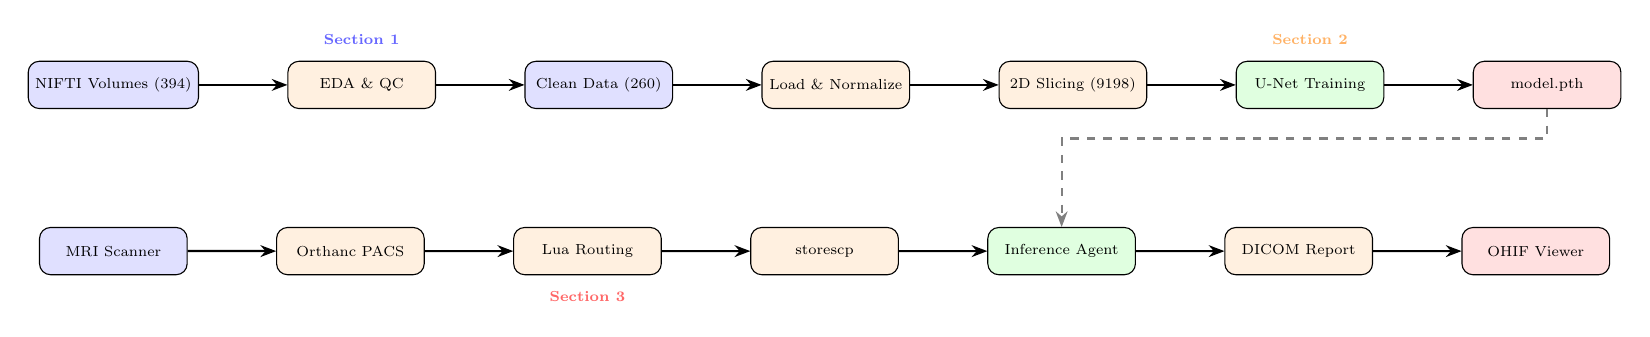
\begin{tikzpicture}[
    scale=0.75, transform shape,
    node distance=0.8cm and 1.5cm,
    box/.style={rectangle, draw, rounded corners, minimum width=2.5cm, minimum height=0.8cm, text centered, font=\scriptsize},
    data/.style={box, fill=blue!12},
    process/.style={box, fill=orange!12},
    model/.style={box, fill=green!12},
    output/.style={box, fill=red!12},
    arrow/.style={-{Stealth[length=2mm]}, thick},
    dashedarrow/.style={-{Stealth[length=2mm]}, thick, dashed, gray}
]

% Section 1
\node[data] (raw) {NIFTI Volumes (394)};
\node[process, right=of raw] (eda) {EDA \& QC};
\node[data, right=of eda] (clean) {Clean Data (260)};

% Section 2
\node[process, right=of clean] (load) {Load \& Normalize};
\node[process, right=of load] (slice) {2D Slicing (9198)};
\node[model, right=of slice] (unet) {U-Net Training};
\node[output, right=of unet] (pth) {model.pth};

% Section 3 (bottom row)
\node[data, below=2cm of raw] (scanner) {MRI Scanner};
\node[process, right=of scanner] (pacs) {Orthanc PACS};
\node[process, right=of pacs] (route) {Lua Routing};
\node[process, right=of route] (listen) {storescp};
\node[model, right=of listen] (infer) {Inference Agent};
\node[process, right=of infer] (report) {DICOM Report};
\node[output, right=of report] (viewer) {OHIF Viewer};

% Arrows row 1
\draw[arrow] (raw) -- (eda);
\draw[arrow] (eda) -- (clean);
\draw[arrow] (clean) -- (load);
\draw[arrow] (load) -- (slice);
\draw[arrow] (slice) -- (unet);
\draw[arrow] (unet) -- (pth);

% Arrows row 2
\draw[arrow] (scanner) -- (pacs);
\draw[arrow] (pacs) -- (route);
\draw[arrow] (route) -- (listen);
\draw[arrow] (listen) -- (infer);
\draw[arrow] (infer) -- (report);
\draw[arrow] (report) -- (viewer);

% Cross-connection
\draw[dashedarrow] (pth.south) -- ++(0,-0.5) -| (infer.north);

% Labels
\node[above=0.15cm of eda, font=\scriptsize\bfseries, color=blue!60] {Section 1};
\node[above=0.15cm of unet, font=\scriptsize\bfseries, color=orange!60] {Section 2};
\node[below=0.15cm of route, font=\scriptsize\bfseries, color=red!60] {Section 3};

\end{tikzpicture}
\caption{End-to-end pipeline architecture. Top: training pathway (Sections 1--2). Bottom: clinical deployment (Section 3). Dashed arrow indicates trained model transfer.}
\label{fig:pipeline}
\end{figure*}

\subsection{Training Configuration}

\begin{table}[H]
\centering
\small
\begin{tabular}{ll}
\toprule
\textbf{Hyperparameter} & \textbf{Value} \\
\midrule
Epochs & 10 \\
Batch size & 8 \\
Learning rate & $2 \times 10^{-4}$ \\
Optimizer & Adam ($\beta_1=0.9, \beta_2=0.999$) \\
Loss & CrossEntropyLoss \\
LR scheduler & ReduceLROnPlateau \\
Training time & 12 min 18 sec \\
\bottomrule
\end{tabular}
\caption{Training hyperparameters}
\end{table}

\subsection{Preprocessing}
\begin{enumerate}[nosep]
    \item \textbf{Intensity normalization}: Min-max scaling to $[0, 1]$
    \item \textbf{Spatial standardization}: Zero-padding to $64 \times 64$ (coronal/sagittal)
    \item \textbf{2D extraction}: Axial slices extracted for 2D U-Net input
\end{enumerate}

\subsection{Evaluation Metrics}

We evaluate using four complementary metrics computed on full 3D volumes:

\textbf{Dice Similarity Coefficient (DSC):}
\begin{equation}
\text{DSC} = \frac{2|P \cap G|}{|P| + |G|}
\end{equation}

\textbf{Jaccard Index (IoU):}
\begin{equation}
J = \frac{|P \cap G|}{|P \cup G|}
\end{equation}

\textbf{Sensitivity (Recall):}
\begin{equation}
\text{Sens} = \frac{TP}{TP + FN}
\end{equation}

\textbf{Specificity:}
\begin{equation}
\text{Spec} = \frac{TN}{TN + FP}
\end{equation}

Additionally, we compute \textbf{per-class Dice scores} for anterior and posterior hippocampus separately.

% ============================================================
% 5. RESULTS
% ============================================================
\section{Results}

\subsection{Training Convergence}

Training loss decreased consistently over 10 epochs, with the model converging to stable low-loss values by epoch 6--7. The learning rate scheduler did not trigger reduction, indicating smooth optimization.

\begin{table}[H]
\centering
\small
\begin{tabular}{cc}
\toprule
\textbf{Epoch} & \textbf{Final Batch Loss} \\
\midrule
0 & 0.0245 \\
3 & 0.0084 \\
6 & 0.0050 \\
9 & 0.0087 \\
\bottomrule
\end{tabular}
\caption{Selected training loss values}
\end{table}

\subsection{Test Set Performance}

\begin{table}[H]
\centering
\small
\begin{tabular}{lc}
\toprule
\textbf{Metric} & \textbf{Value} \\
\midrule
Mean Dice & \textbf{0.9001} \\
Mean Jaccard & \textbf{0.8195} \\
Mean Sensitivity & $\sim$0.89 \\
Mean Specificity & $\sim$0.998 \\
Best Dice & 0.9368 \\
Worst Dice & 0.8229 \\
\bottomrule
\end{tabular}
\caption{Test set results across 52 volumes}
\label{tab:results}
\end{table}

\subsection{Per-Volume Analysis}

The Dice score distribution is concentrated in the 0.88--0.93 range with only 4 volumes below 0.85. The worst-performing volumes (Dice $\approx$ 0.82) exhibit smaller hippocampal regions, ambiguous anterior-posterior boundaries, or lower image quality.

\begin{table}[H]
\centering
\small
\begin{tabular}{lcc}
\toprule
\textbf{Volume} & \textbf{Dice} & \textbf{Jaccard} \\
\midrule
\multicolumn{3}{c}{\textit{Top 5}} \\
hippocampus\_146 & 0.937 & 0.881 \\
hippocampus\_034 & 0.933 & 0.874 \\
hippocampus\_175 & 0.932 & 0.873 \\
hippocampus\_207 & 0.931 & 0.871 \\
hippocampus\_152 & 0.930 & 0.870 \\
\midrule
\multicolumn{3}{c}{\textit{Bottom 5}} \\
hippocampus\_070 & 0.858 & 0.752 \\
hippocampus\_042 & 0.832 & 0.712 \\
hippocampus\_125 & 0.827 & 0.705 \\
hippocampus\_305 & 0.826 & 0.703 \\
hippocampus\_334 & 0.823 & 0.699 \\
\bottomrule
\end{tabular}
\caption{Best and worst performing test volumes}
\end{table}

\subsection{Clinical Deployment Validation}

The deployed system was validated against three test studies containing complete DICOM brain MRI examinations with multiple series. The system correctly:
\begin{itemize}[nosep]
    \item Identified the HippoCrop series from multi-series studies
    \item Constructed 3D volumes from unordered DICOM files
    \item Generated volumetric measurements
    \item Produced DICOM-compliant reports sent back to PACS
\end{itemize}

% ============================================================
% 6. CLINICAL INTEGRATION
% ============================================================
\section{Clinical Integration}

\subsection{DICOM Report Generation}

The system generates a $1000 \times 1000$ RGB DICOM Secondary Capture image containing:
\begin{itemize}[nosep]
    \item Patient identification metadata
    \item Anterior, posterior, and total hippocampal volumes (mm\textsuperscript{3})
    \item Clinical range assessment (2,500--4,500 mm\textsuperscript{3} reference)
    \item Three representative axial slices with segmentation overlay (green=anterior, red=posterior)
    \item AI model information and disclaimer
\end{itemize}

The report is stored as a DICOM Secondary Capture (SOP Class 1.2.840.10008.5.1.4.1.1.7) with all mandatory modules per DICOM PS3.3 Section A.8 (Patient, Study, Series, Equipment, SC Equipment, Image Pixel, SOP Common).

\subsection{Deployment Architecture}

The clinical integration uses:
\begin{enumerate}[nosep]
    \item \textbf{Orthanc} as the PACS server (port 4242)
    \item \textbf{Lua script} for automatic routing of incoming studies
    \item \textbf{DCMTK storescp} as the AI listener (port 106)
    \item \textbf{CPU-only PyTorch} inference ($<5$ sec/volume)
    \item \textbf{DCMTK storescu} to return results to PACS
\end{enumerate}

% ============================================================
% 7. DISCUSSION
% ============================================================
\section{Discussion}

\subsection{Performance Context}
Our mean Dice of 0.900 is competitive with published results on the Medical Decathlon Hippocampus dataset. The 2D slice-by-slice approach, while simpler than 3D methods, achieves strong performance due to the small, homogeneous nature of hippocampal crop volumes.

\subsection{Limitations}
\begin{itemize}[nosep]
    \item \textbf{2D approach}: Lacks inter-slice context; a 3D U-Net could capture volumetric continuity
    \item \textbf{No data augmentation}: Adding rotation, elastic deformation, and intensity changes would improve robustness
    \item \textbf{Fixed normalization}: Per-volume max normalization; percentile-based or standardization may be more robust
    \item \textbf{No cross-validation}: Single fixed split; k-fold would give more reliable estimates
\end{itemize}

\subsection{Future Work}
\begin{itemize}[nosep]
    \item 3D U-Net or hybrid 2.5D approach
    \item Dice + Cross-Entropy combined loss
    \item Test-time augmentation (TTA) for improved worst-case performance
    \item Multi-site validation
    \item Longitudinal tracking (serial volume changes per patient)
\end{itemize}

% ============================================================
% 8. CONCLUSION
% ============================================================
\section{Conclusion}

We presented HippoVolume.AI, a complete end-to-end system for automated hippocampal volume quantification from brain MRI. The system achieves a mean Dice coefficient of 0.900 on a held-out test set, demonstrating clinical-grade segmentation performance. The full DICOM/PACS integration enables seamless deployment into existing clinical workflows, with automated report generation and sub-5-second inference times on standard CPU hardware.

% ============================================================
% REFERENCES
% ============================================================
\begin{thebibliography}{10}
\small

\bibitem{who2019}
World Health Organization,
\textit{Dementia Key Facts},
2019.

\bibitem{jack2010}
Jack, C.R. Jr. et al.,
``Hypothetical model of dynamic biomarkers of the Alzheimer's pathological cascade,''
\textit{The Lancet Neurology}, vol. 9, no. 1, pp. 119--128, 2010.

\bibitem{ronneberger2015}
Ronneberger, O., Fischer, P., and Brox, T.,
``U-Net: Convolutional Networks for Biomedical Image Segmentation,''
\textit{MICCAI}, pp. 234--241, 2015.

\bibitem{cicek2016}
\c{C}i\c{c}ek, \"{O}. et al.,
``3D U-Net: Learning Dense Volumetric Segmentation from Sparse Annotation,''
\textit{MICCAI}, pp. 424--432, 2016.

\bibitem{milletari2016}
Milletari, F., Navab, N., and Ahmadi, S.-A.,
``V-Net: Fully Convolutional Neural Networks for Volumetric Medical Image Segmentation,''
\textit{3DV}, pp. 565--571, 2016.

\bibitem{oktay2018}
Oktay, O. et al.,
``Attention U-Net: Learning Where to Look for the Pancreas,''
\textit{MIDL}, 2018.

\bibitem{thyreau2018}
Thyreau, B. et al.,
``Segmentation of the hippocampus by transferring algorithmic knowledge for large cohort processing,''
\textit{Medical Image Analysis}, vol. 43, pp. 214--228, 2018.

\bibitem{liu2020}
Liu, M. et al.,
``A multi-model deep convolutional neural network for automatic hippocampus segmentation and classification in Alzheimer's disease,''
\textit{NeuroImage}, vol. 208, p. 116459, 2020.

\end{thebibliography}

\end{document}
